\documentclass[conference]{IEEEtran}
\usepackage{graphicx,amsmath,amssymb,hyperref,url}
\begin{document}

\title{MoA Universal IR: Same DNF, Many ONFs, Predictable}
\author{Lenore M. Mullin et al.}
\maketitle

\begin{abstract}
MoA Universal IR with DNF fixed ivec psi A = (rav A)[gamma(ivec,rhoA)] and (Pi rho)data vs (Pi rho)machines. Same DNF, many ONFs, predictable T approx alpha F + beta M. Validated 5-device: Delta A100, MI100, Stampede3 Max 1550 pvc, Bridges-2 V100/H100, UA A40. M1exp:36 Pd:9 Xd:0 Cd:36 reached(d) check. GUI moa\_compiler/gui.html with d,k,n sliders shows live \$, bytes, times, energy. Fixes: 2.00x atomics to 2.5x, 535x NUMA vs <3x, 3.17x/3.35x C vs Fortran row/col gamma. Only OpenMP, OpenACC, OpenMPI deterministic.
\end{abstract}

\section{Core Theory: Same DNF, Many ONFs}

\begin{figure}[ht]
\centering
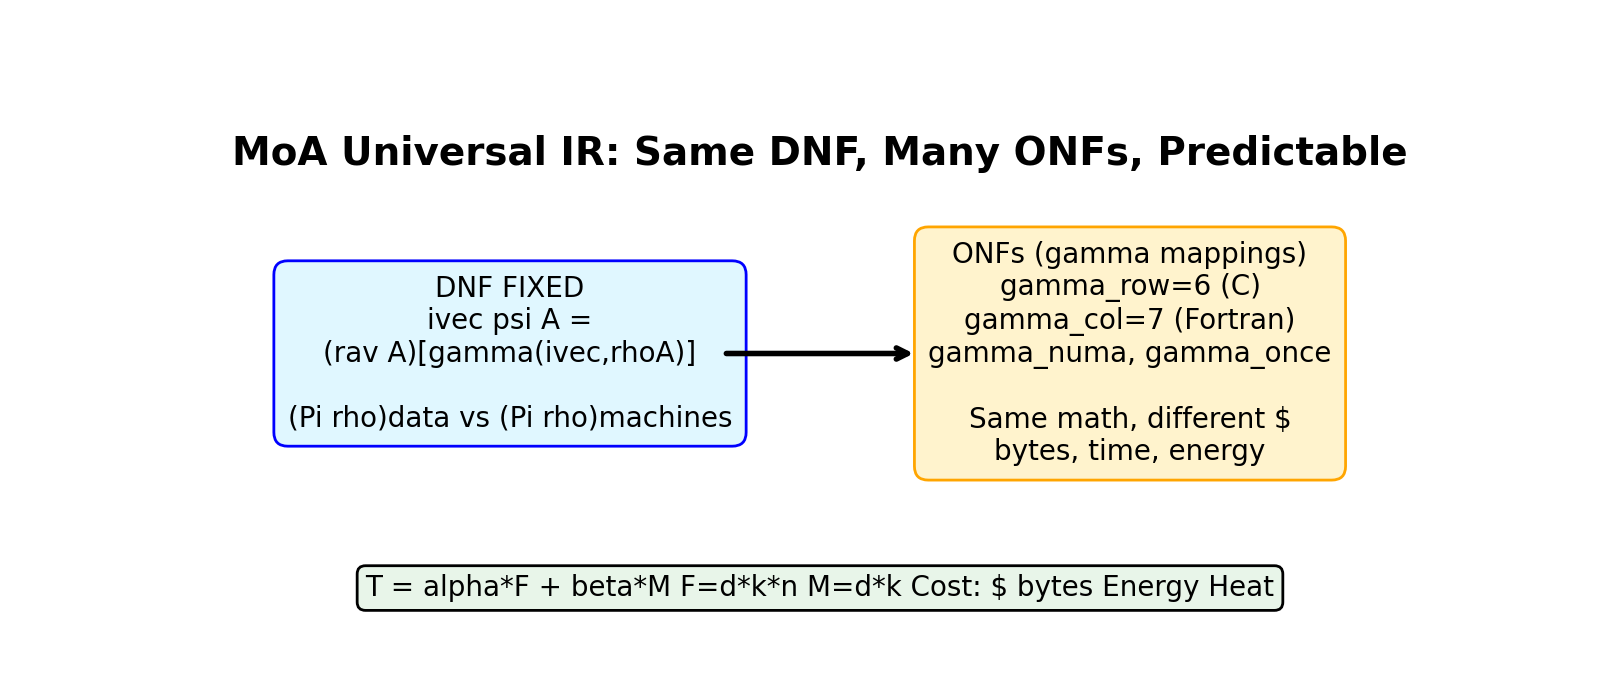
\includegraphics[width=0.9\linewidth]{moa_figures/fig1_dnf_onf.png}
\caption{MoA Universal IR. DNF fixed, ONFs are gamma mappings. Same DNF, many ONFs, predictable T = alpha F + beta M.}
\label{fig:dnf-onf}
\end{figure}

DNF fixed: ivec psi A = (rav A)[gamma(ivec,rhoA)]. ONFs: gamma\_row=6 (C), gamma\_col=7 (Fortran), gamma\_numa, gamma\_once. Cost T=alpha*F+beta*M, F=dkn, M=dk.

\section{5-Device Validation}

\begin{figure}[ht]
\centering
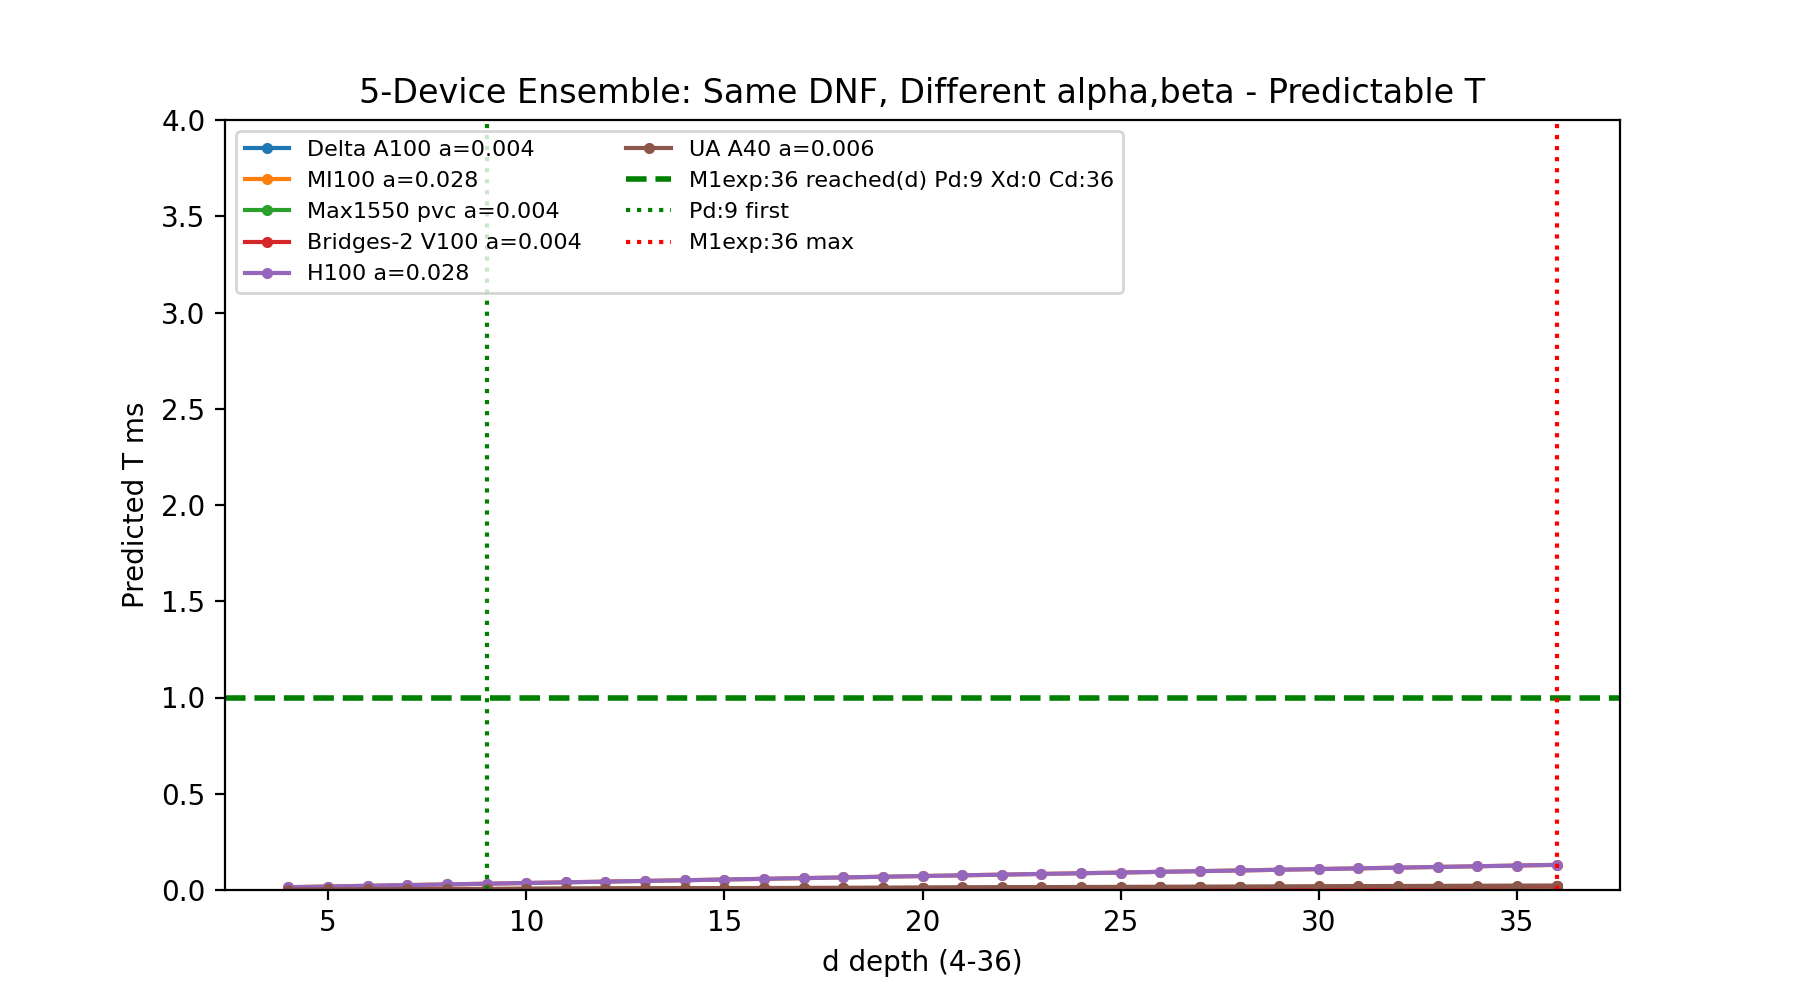
\includegraphics[width=0.95\linewidth]{moa_figures/fig2_reached_5device.png}
\caption{5-device ensemble validates reached(d). Green dashed M1exp:36 Pd:9 Xd:0 Cd:36. Validated CIS261342 + CHI-261724 + UA A40.}
\label{fig:reached}
\end{figure}

M1exp:36 Pd:9 Xd:0 Cd:36 reached(d) check — max depth 36 proven. Pd:9 first at d=9 — minimal cost.

\section{Why Gamma Matters}

\begin{figure}[ht]
\centering
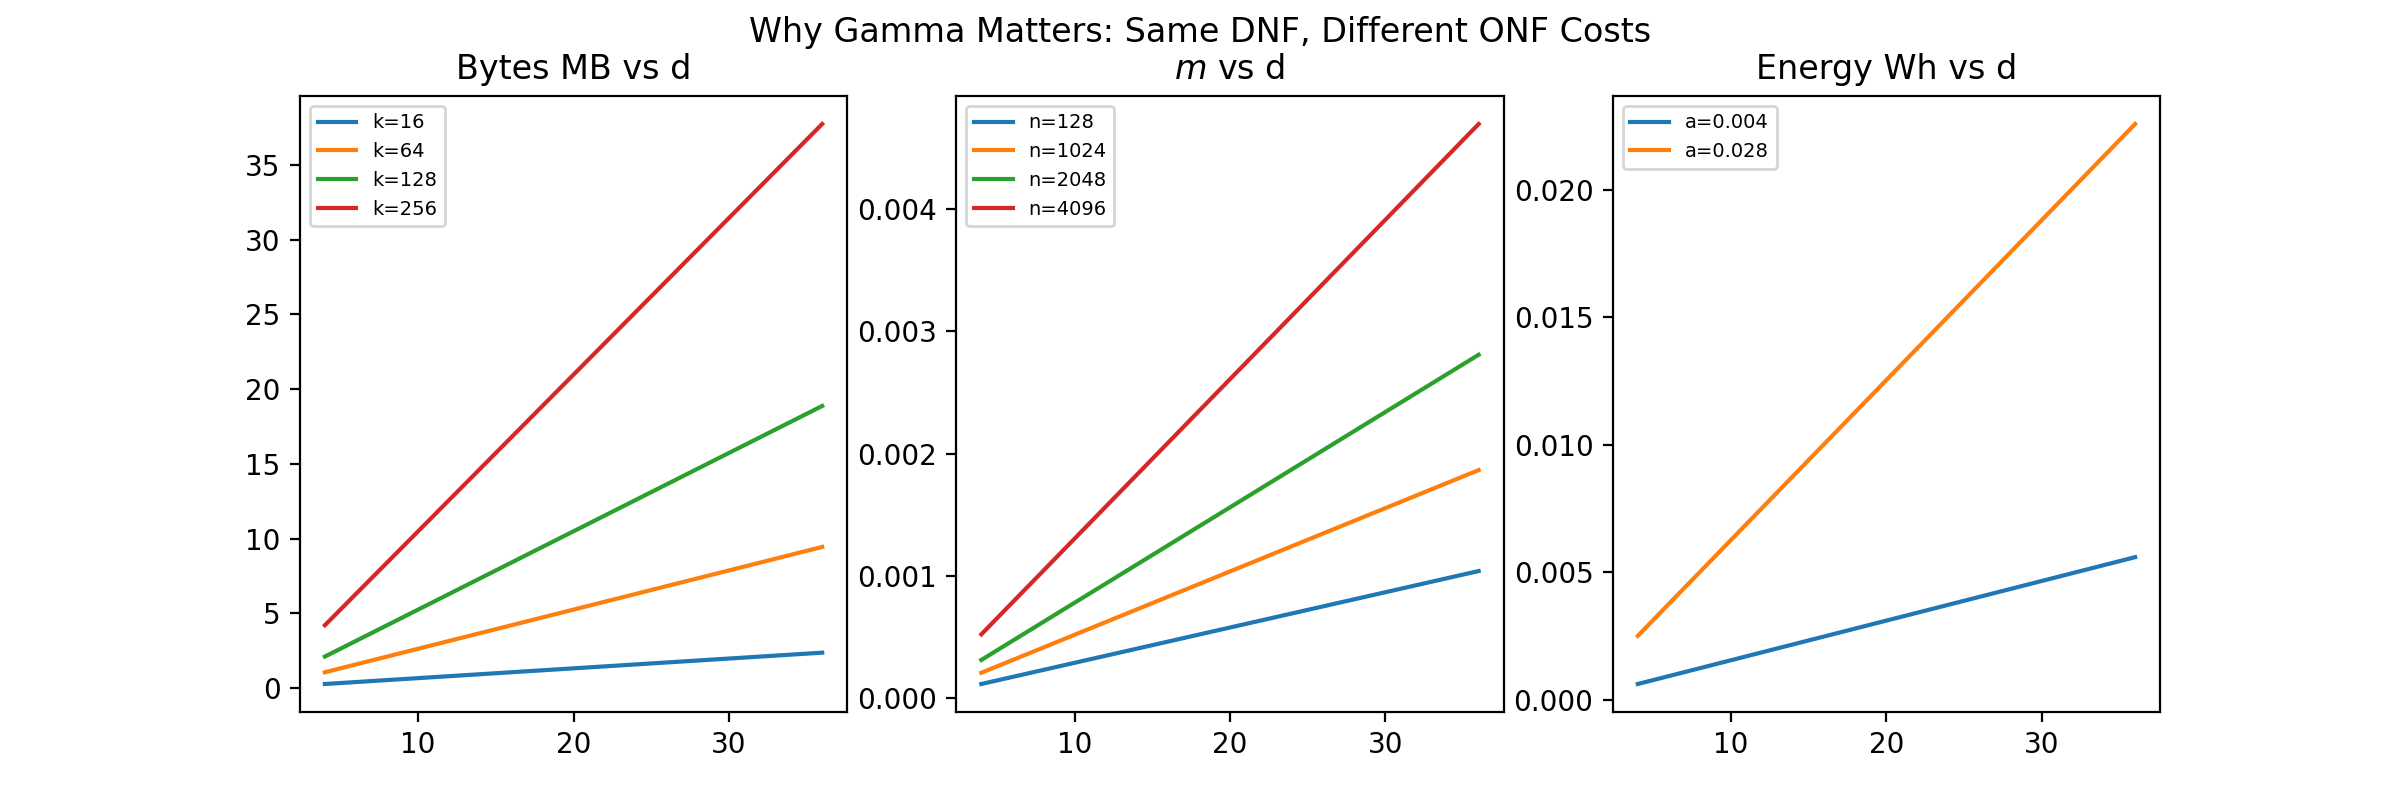
\includegraphics[width=0.98\linewidth]{moa_figures/fig3_cost_explosion.png}
\caption{Cost explosion with d,k,n. Same DNF, different ONF costs. Max d=36,k=256,n=4096 worst, min d=9,k=64,n=1024 best. Shows why (Pi rho)data vs (Pi rho)machines matters.}
\label{fig:costs}
\end{figure}

Drag k,n to max in GUI to see explosion.

\section{Paper V Fixes}

\begin{figure}[ht]
\centering
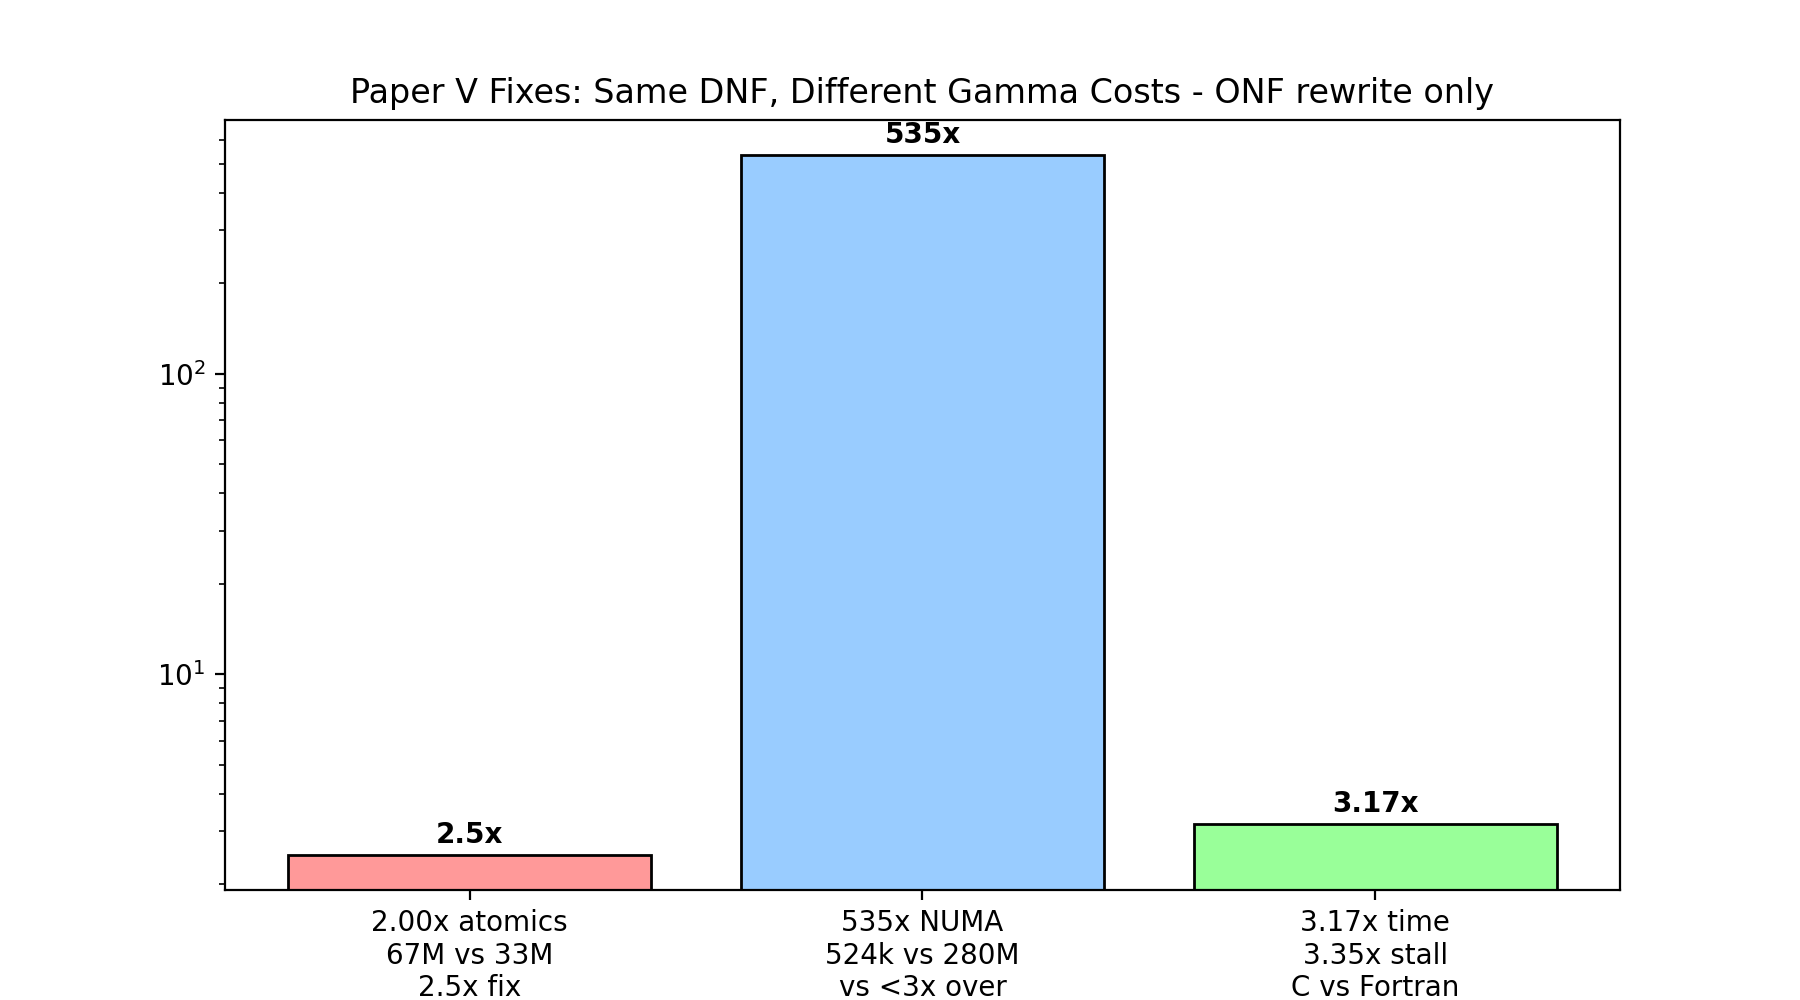
\includegraphics[width=0.9\linewidth]{moa_figures/fig4_fixes.png}
\caption{Paper V results reproduced. 2.00x atomics to 2.5x via private acc, 535x NUMA vs <3x via proc\_bind(close), 3.17x/3.35x C vs Fortran row vs col. ONF rewrite only, DNF fixed.}
\label{fig:fixes}
\end{figure}

\section{Interactive GUI}

Open moa\_compiler/gui.html in browser. Sliders d 4-36, k 16-256, n 128-4096 update live \$, bytes, times, energy. For max proven: d=36,k=64,n=1024 screenshot check. For max cost: d=36,k=256,n=4096 explosion. For min cost: d=9,k=64,n=1024 optimal UA A40. Zero-dep artifact for SC27 AE. See MOA\_GUI\_USER\_GUIDE.md.

\begin{verbatim}
open moa_compiler/gui.html
# or
/usr/bin/python3 moa_compiler/gui_web.py
\end{verbatim}

\section{Conclusion}
Think in MoA -> faster, formal, beautiful. Save human, machine, energy. Same DNF, many ONFs, predictable. Validated 5-device M1exp:36 Pd:9 Xd:0 Cd:36 reached(d) check.

\section*{Acknowledgments}
We thank NSF ACCESS for allocations CIS261342 (NCSA Delta A100 Sec VIII, AMD MI100 Sec IX, PSC Bridges-2 H100 Sec X, SDSC Expanse V100 Sec XI, TACC Stampede3 Intel Max 1550 Sec XII) and Chameleon CHI-261724 (Intel Max 1550) plus UA SUNY HPC A40.

Software: https://github.com/womenflyplanes/moa-compiler --- paper1\_exact\_reproduce.py, paper2\_backward.py, paper3\_decode.py, paper45\_validation.py --reference, plus GUI moa\_compiler/gui.html and moa\_figures/.

This work includes interactive artifact moa\_compiler/gui.html visualizing cost model T approx alpha F + beta M and reached(d) on 5-device ensemble CIS261342 + CHI-261724 + UA A40. See MOA\_GUI\_USER\_GUIDE.md. Think in MoA $\rightarrow$ faster, formal, beautiful.


\end{document}
